%\documentclass[a4paper]{article}
\documentclass[11pt,a4paper]{article}
\usepackage[swedish]{babel}  % swedish use the next line as well
\usepackage[utf8]{inputenc}
%\usepackage[cm]{fullpage}
%\usepackage{fullpage}
%\usepackage{a4wide}


\usepackage{graphicx}
\usepackage{tocloft}
\usepackage{pgf,tikz}
\usetikzlibrary{arrows}
%\usepackage{lastpage}

\begin{document}
%\raggedright

% Formatering av framsida

\begin{titlepage}

\includegraphics[height=2.0cm]{mah_logo.eps}
\begin{center}
  
% Upper part of the page. The '~' is needed because \\
% only works if a paragraph has started.
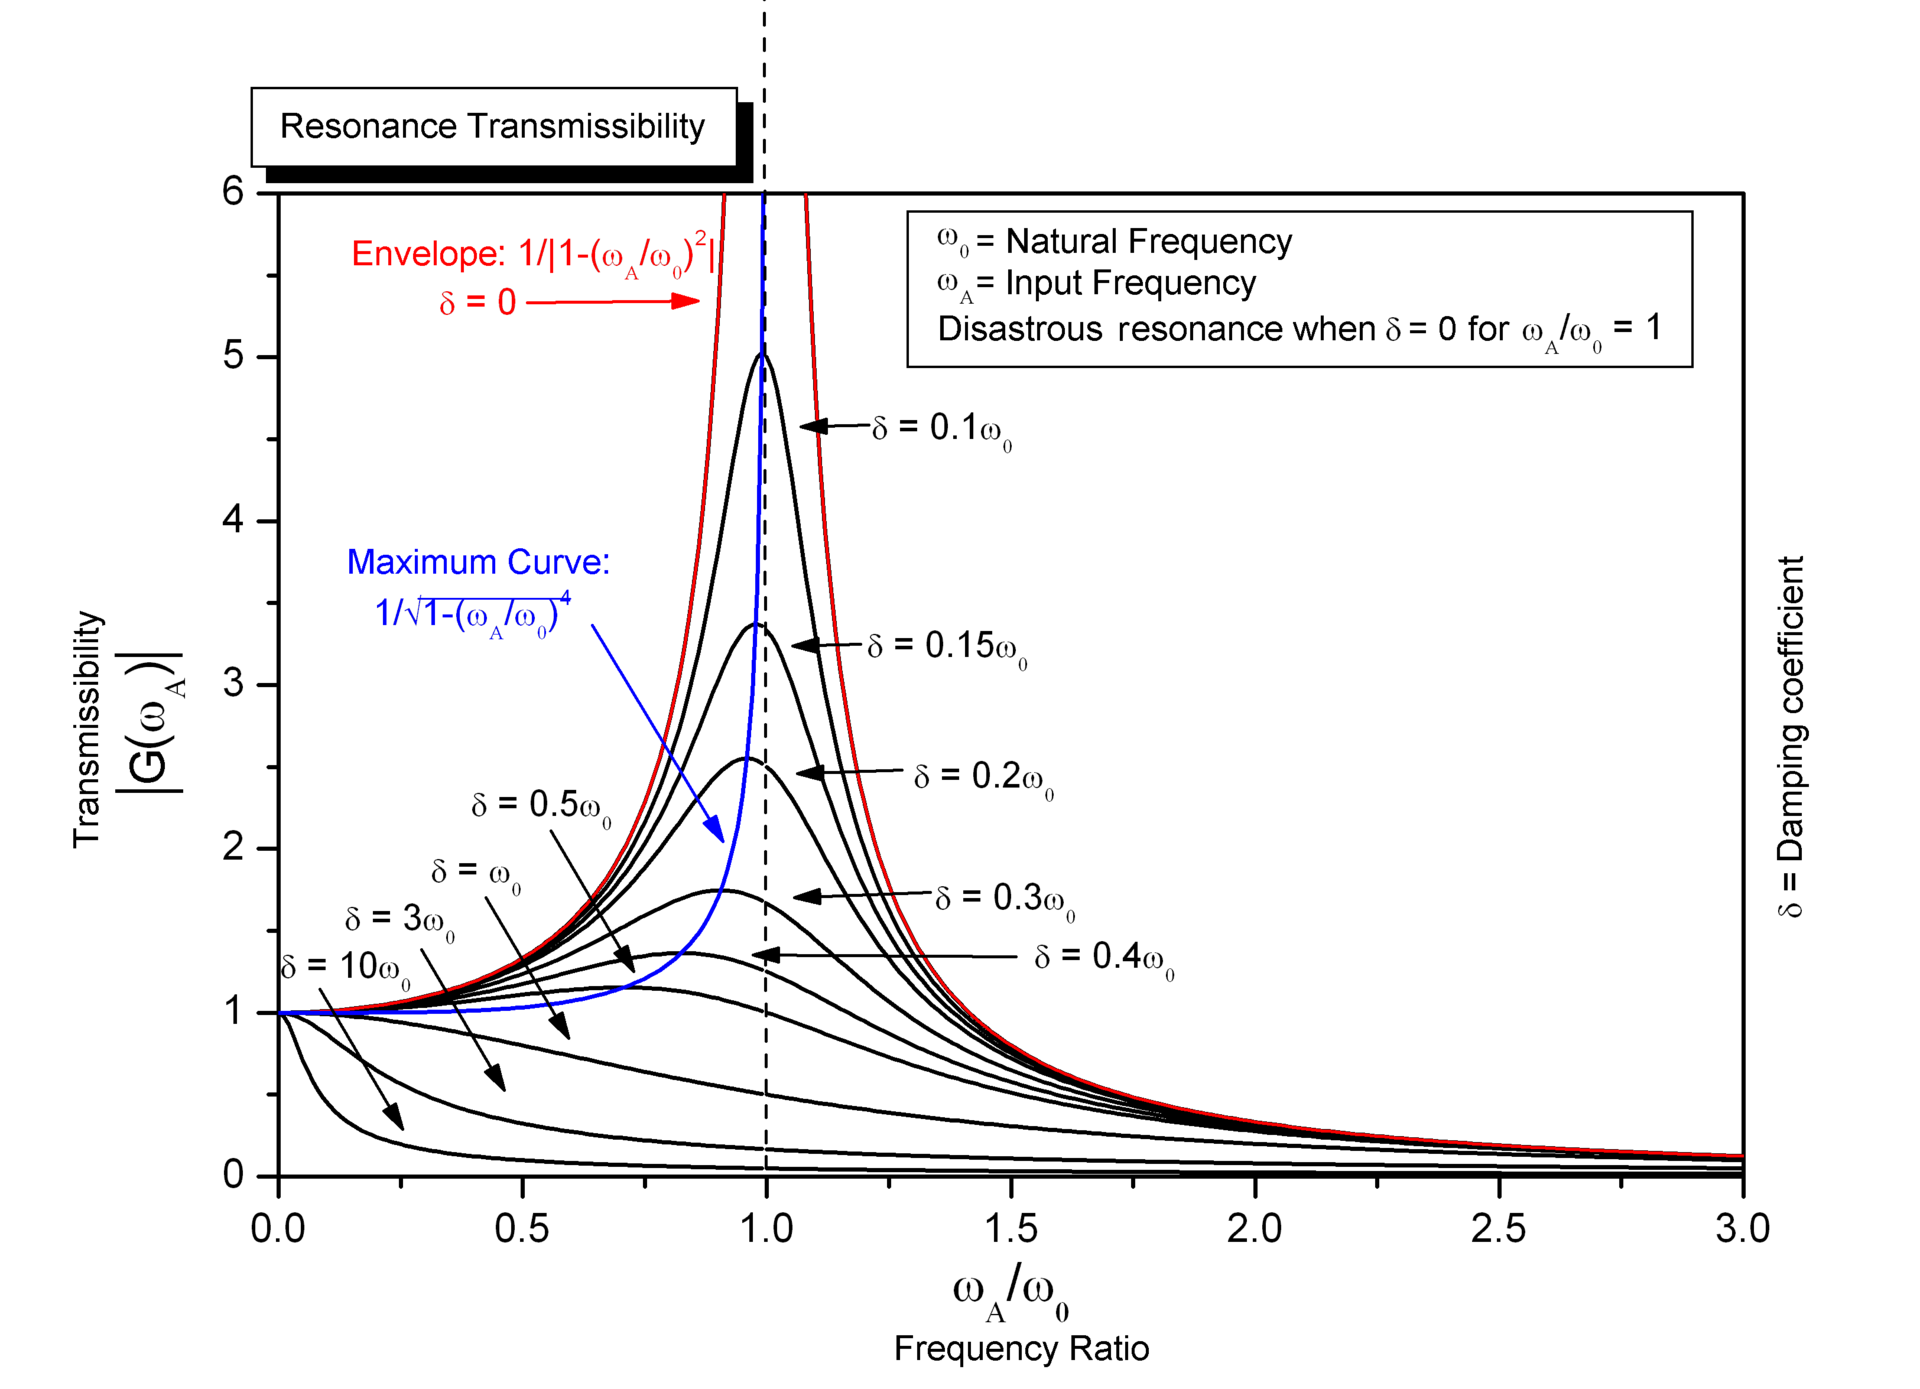
\includegraphics[width=0.15\textwidth]{./fig1.png}~\\[1cm]

{\LARGE Arbetsuppgift \#:\\ [0.2cm]}

{\Large eventuell undertitel\\ [1.0cm]}

\begin{flushright}
Modeller och verklighet, Datateknik, HT15 \\
\end{flushright}
\vfill
\begin{flushleft}
  {\bf Grupp:} \#\# \\
  {\bf Namn:} Förnamn Efternamn \\
  {\bf Namn:} Förnamn Efternamn \\
  {\bf Namn:} Förnamn Efternamn \\
  {\bf Namn:} Förnamn Efternamn \\
  ~\\
  Datum för inlämning: ÅÅMMDD \\
  ~\\
  Status:\\
  \vspace{5mm}

  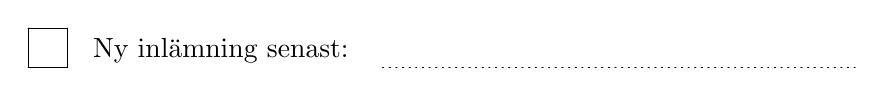
\begin{tikzpicture}[line cap=round,line join=round,>=triangle 45,x=1.0mm,y=1.0mm]
\draw (-5,10)-- (0,10);
\draw (0,10)-- (0,5);
\draw (0,5)-- (-5,5);
\draw (-5,5)-- (-5,10);
\draw (2,10) node[anchor=north west] {Ny inlämning senast:};
\draw [dotted] (40,5)-- (100,5);
\end{tikzpicture}\\

  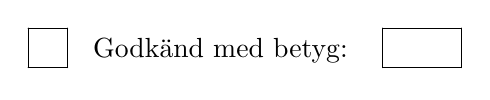
\begin{tikzpicture}[line cap=round,line join=round,>=triangle 45,x=1.0mm,y=1.0mm]
\draw (-5,10)-- (0,10);
\draw (0,10)-- (0,5);
\draw (0,5)-- (-5,5);
\draw (-5,5)-- (-5,10);
\draw (2,10) node[anchor=north west] {Godkänd med betyg:};
\draw (40,10)-- (50,10);
\draw (50,10)-- (50,5);
\draw (50,5)-- (40,5);
\draw (40,5)-- (40,10);
\end{tikzpicture}\\

  
\begin{tikzpicture}[line cap=round,line join=round,>=triangle 45,x=1.0mm,y=1.0mm]
    \draw (-5,10)-- (0,10);
    \draw (0,10)-- (0,5);
    \draw (0,5)-- (-5,5);
    \draw (-5,5)-- (-5,10);
    \draw (2,10) node[anchor=north west] {Underkänd på grund av:};
    \draw [dotted] (47,5)-- (120,5);
  \end{tikzpicture}\\

  \begin{tikzpicture}[line cap=round,line join=round,>=triangle 45,x=1.0mm,y=1.0mm]
    \draw [dotted] (-5,5)-- (120,5);
  \end{tikzpicture}\\
  \vspace{5mm}

  Lärarens underskrift: \\
  ~\\
  Datum: \\
  ~\\
  Ansvarig lärare: Jörgen Ekman\\
  ~\\
  Kommentarer: 
\end{flushleft}

%\vfill
\end{center}
\end{titlepage}



\tableofcontents

\newpage
\section*{Förord}
\addcontentsline{toc}{section}{\protect\numberline{}Förord}%

Lorem ipsum dolor sit amet, consectetur adipiscing elit. Aenean
consequat, tellus non mollis sodales, massa eros Malmö högskola
tincidunt sapien, in consequat tortor lorem id elit. Cras vitae lorem
eget magna laoreet commodo. Nam euismod mi sit amet metus commodo ac
mattis turpis suscipit.

\newpage
\section{Inledning}
\subsection{Bakgrund}
Lorem ipsum dolor sit amet, consectetur adipiscing elit. Aenean
consequat, tellus non mollis sodales, massa eros tincidunt sapien, in
consequat tortor lorem id elit. Cras vitae lorem eget magna laoreet
commodo. Nam euismod mi sit amet metus commodo ac mattis turpis
suscipit. Proin malesuada elit eget ipsum bibendum tempor. Praesent
vel ullamcorper purus. Nulla pretium viverra dui, pharetra auctor nisl
iaculis iaculis. Aliquam erat volutpat. Ut mollis imperdiet lorem, vel
luctus tortor semper a. Fusce interdum neque vel mauris tincidunt
gravida. Donec volutpat dui sit amet mauris malesuada varius. Som ses
i figur~\ref{fig1}.


\begin{figure}[hbt]
  \begin{center}
    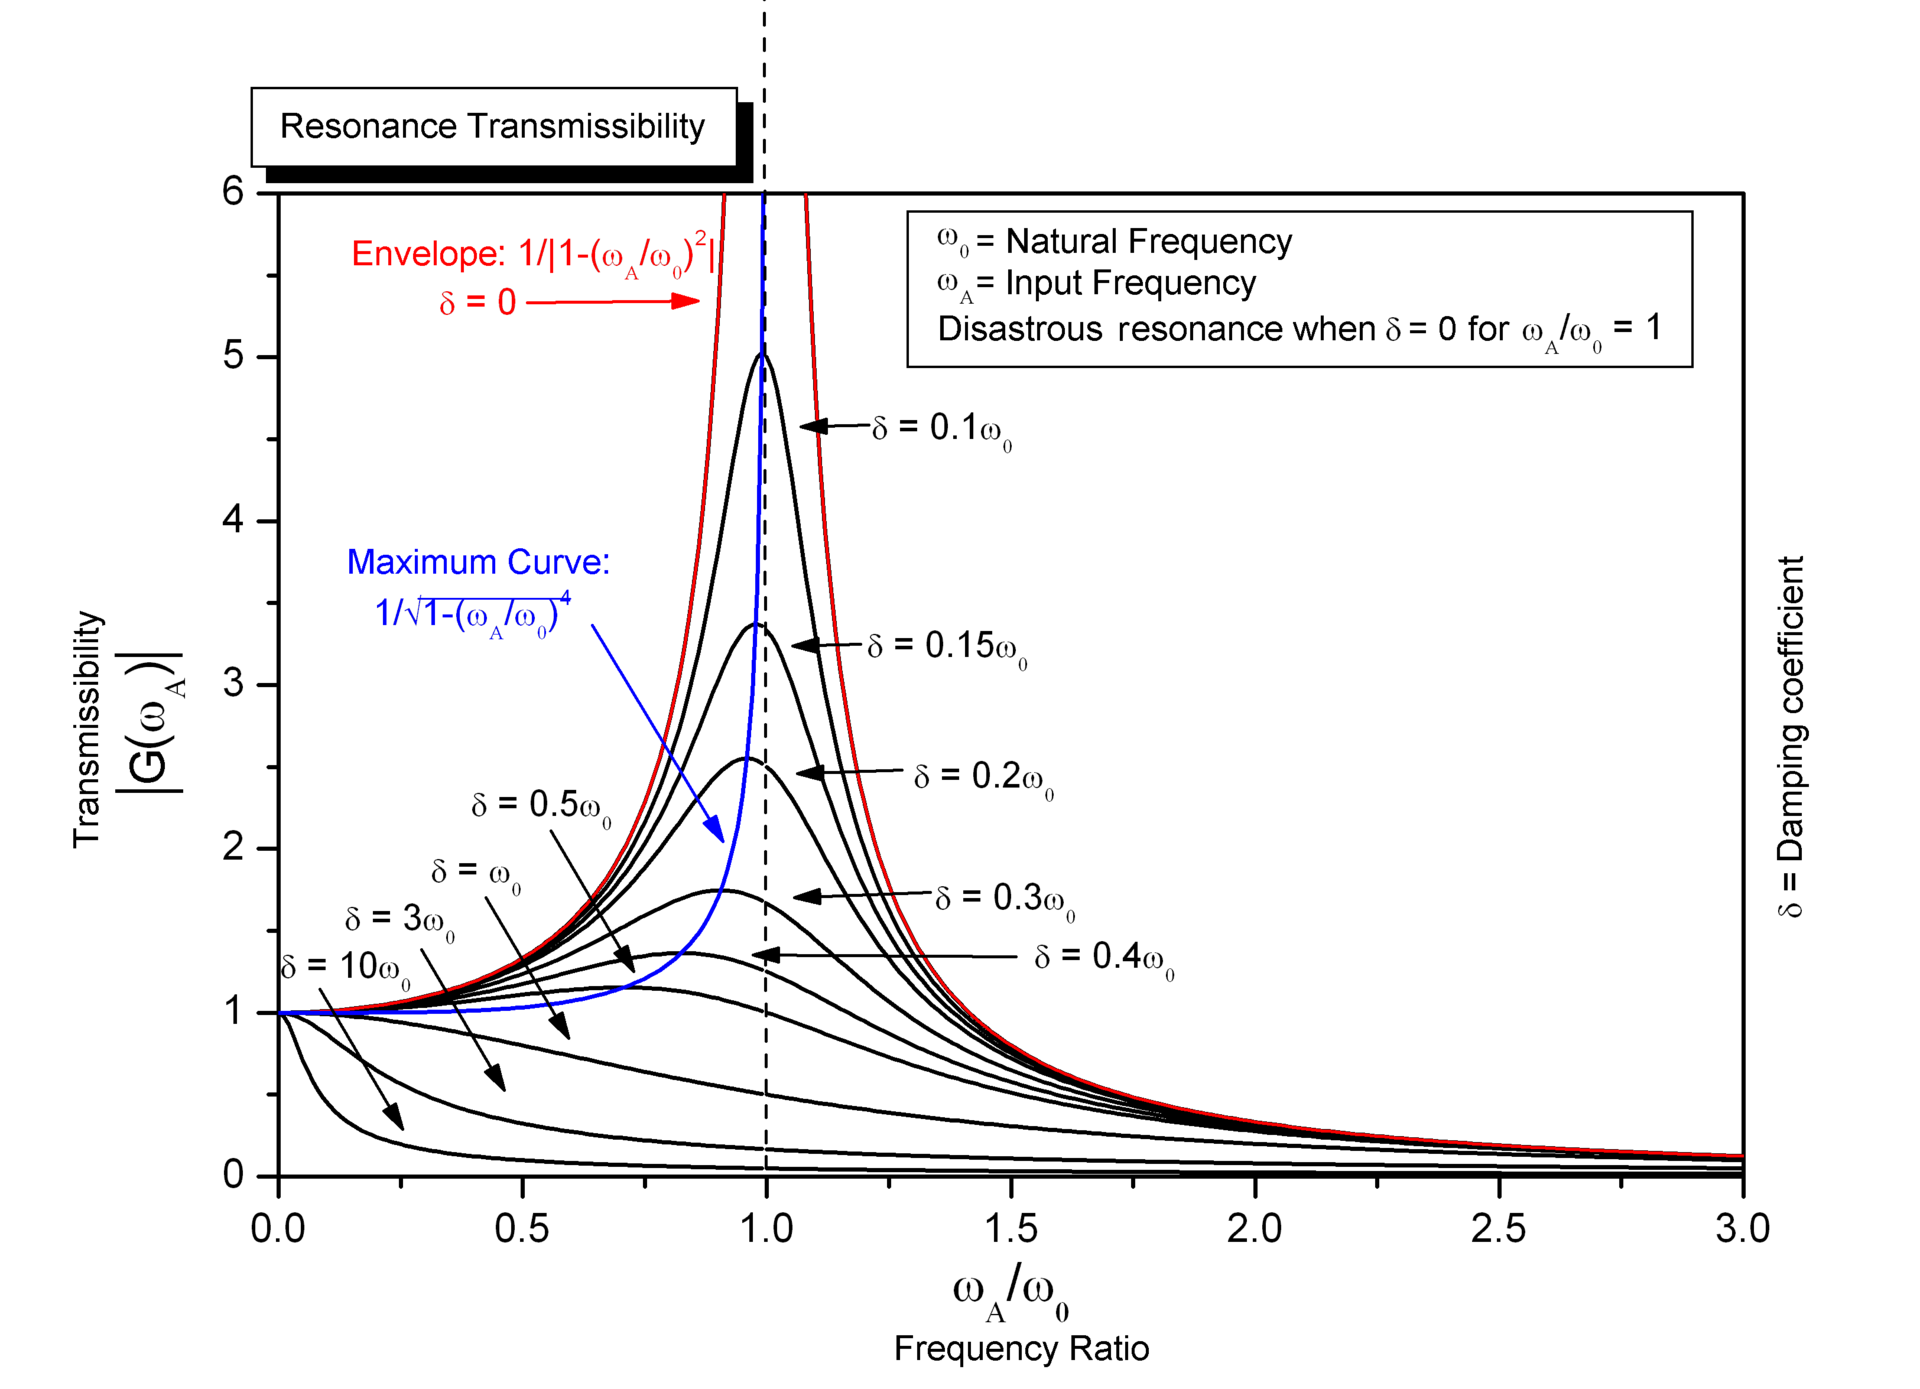
\includegraphics[width=3cm,angle=0]{fig1.png}
    \caption{Marcus Tullius Cicero.}
    \label{fig1}
  \end{center}
\end{figure}

Quisque sit amet erat et eros blandit luctus vitae sagittis nibh. Sed
pharetra dignissim quam eu hendrerit. Morbi vulputate vehicula mi eu
tincidunt.

\subsection{Problemformulering}
Lorem ipsum dolor sit amet, consectetur adipiscing elit. Aenean
consequat, tellus non mollis sodales, massa eros tincidunt sapien, in
consequat tortor lorem id elit. Cras vitae lorem eget magna laoreet
commodo~\cite{bib:mattson.2008}. Nam euismod mi sit amet metus commodo
ac mattis turpis suscipit. Proin malesuada elit eget ipsum bibendum
tempor. Praesent vel ullamcorper purus. Nulla pretium viverra dui,
pharetra auctor nisl iaculis iaculis. Aliquam erat volutpat. Ut mollis
imperdiet lorem, vel luctus tortor semper a. Fusce interdum neque vel
mauris tincidunt gravida. Donec volutpat dui sit amet mauris malesuada
varius.

\begin{equation}
  x=\frac{-b\pm \sqrt{b^2-4ac}}{2a}
\end{equation}

Quisque sit amet erat et eros blandit luctus vitae sagittis nibh. Sed
pharetra dignissim quam eu hendrerit~\cite{bib:persson.2010.01}. Morbi
vulputate vehicula mi eu tincidunt.

\subsection{Syfte och avgränsningar}
Lorem ipsum dolor sit amet, consectetur adipiscing elit. Aenean
consequat, tellus non mollis sodales, massa eros tincidunt sapien, in
consequat tortor lorem id elit. Cras vitae lorem eget magna laoreet
commodo. Nam euismod mi sit amet metus commodo ac mattis turpis
suscipit. Proin malesuada elit eget ipsum bibendum tempor. Praesent
vel ullamcorper purus. Nulla pretium viverra dui, pharetra auctor nisl
iaculis iaculis. Aliquam erat volutpat. Ut mollis imperdiet lorem, vel
luctus tortor semper a. Fusce interdum neque vel mauris tincidunt
gravida. Donec volutpat dui sit amet mauris malesuada varius. Quisque
sit amet erat et eros blandit luctus vitae sagittis nibh. Sed pharetra
dignissim quam eu hendrerit. Morbi vulputate vehicula mi eu tincidunt.

\subsection{Metod och genomförande}
Lorem ipsum dolor sit amet, consectetur adipiscing elit. Aenean
consequat, tellus non mollis sodales, massa eros tincidunt sapien, in
consequat tortor lorem id elit. Cras vitae lorem eget magna laoreet
commodo. Nam euismod mi sit amet metus commodo ac mattis turpis
suscipit. Proin malesuada elit eget ipsum bibendum tempor. Praesent
vel ullamcorper purus. Nulla pretium viverra dui, pharetra auctor nisl
iaculis iaculis. Aliquam erat volutpat. Ut mollis imperdiet lorem, vel
luctus tortor semper a. Fusce interdum neque vel mauris tincidunt
gravida. Donec volutpat dui sit amet mauris malesuada varius.

\begin{table}[hbt]
  \begin{center}
    \caption{Några mesar i Sverige.}
    \label{mesar}
    \begin{tabular}{|l|l|l|}
      \hline
      Art      & Artnamn         & Förekomst i Sverige \\
      \hline
      Azurmes  & Parus cyanus    & Tillfällig \\
      \hline
      Blåmes   & Parus caeruleus & Allmän \\
      \hline
      Entita   & Parus palustris & Sällsynt \\ 
      \hline
      Talltita & Parus montanus  & Allmän \\
      \hline
    \end{tabular}
  \end{center}
\end{table}

\subsubsection*{Rubrik i tredje graden}
\addcontentsline{toc}{subsection}{\protect\numberline{}Rubrik i tredje graden} 
Quisque sit amet erat et eros blandit luctus vitae sagittis
nibh. Sed pharetra dignissim quam eu hendrerit. Morbi vulputate
vehicula mi eu tincidunt.

\subsubsection*{Rubrik i tredje graden igen}
\addcontentsline{toc}{subsection}{\protect\numberline{}Rubrik i tredje graden igen}
Som ses i tabell~\ref{mesar}. Quisque sit amet erat et eros blandit
luctus vitae sagittis nibh. Sed pharetra dignissim quam eu
hendrerit. Morbi vulputate vehicula mi eu tincidunt.

\subsection{Disposition}
Lorem ipsum dolor sit amet, consectetur adipiscing elit. Aenean
consequat, tellus non mollis sodales, massa eros tincidunt sapien, in
consequat tortor lorem id elit. Cras vitae lorem eget magna laoreet
commodo. Nam euismod mi sit amet metus commodo ac mattis turpis
suscipit. Proin malesuada elit eget ipsum bibendum tempor. Praesent
vel ullamcorper purus. Nulla pretium viverra dui, pharetra auctor nisl
iaculis iaculis. Aliquam erat volutpat.

\newpage
\section{Andra kapitlet}
Lorem ipsum dolor sit amet, consectetur adipiscing elit. Aenean
consequat, tellus non mollis sodales, massa eros tincidunt sapien, in
consequat tortor lorem id elit. Cras vitae lorem eget magna laoreet
commodo. Nam euismod mi sit amet metus commodo ac mattis turpis
suscipit. Proin malesuada elit eget ipsum bibendum tempor. Praesent
vel ullamcorper purus. Nulla pretium viverra dui, pharetra auctor nisl
iaculis iaculis. Aliquam erat volutpat. Ut mollis imperdiet lorem, vel
luctus tortor semper a. Fusce interdum neque vel mauris tincidunt
gravida. Donec volutpat dui sit amet mauris malesuada varius. Quisque
sit amet erat et eros blandit luctus vitae sagittis nibh. Sed pharetra
dignissim quam eu hendrerit. Morbi vulputate vehicula mi eu tincidunt.

\newpage
\section{Tredje kapitlet}
Lorem ipsum dolor sit amet, consectetur adipiscing elit. Aenean
consequat, tellus non mollis sodales, massa eros tincidunt sapien, in
consequat tortor lorem id elit. Cras vitae lorem eget magna laoreet
commodo. Nam euismod mi sit amet metus commodo ac mattis turpis
suscipit. Proin malesuada elit eget ipsum bibendum tempor. Praesent
vel ullamcorper purus. Nulla pretium viverra dui, pharetra auctor nisl
iaculis iaculis. Aliquam erat volutpat. Ut mollis imperdiet lorem, vel
luctus tortor semper a. Fusce interdum neque vel mauris tincidunt
gravida.

Donec volutpat dui sit amet mauris malesuada varius. Quisque sit amet
erat et eros blandit luctus vitae sagittis nibh. Sed pharetra
dignissim quam eu hendrerit. Morbi vulputate vehicula mi eu tincidunt

Nulla pretium viverra dui, pharetra auctor nisl iaculis
iaculis. Aliquam erat volutpat. Ut mollis imperdiet lorem, vel luctus
tortor semper a. Fusce interdum neque vel mauris tincidunt
gravida. Donec volutpat dui sit amet mauris malesuada varius. Quisque
sit amet erat et eros blandit luctus vitae sagittis nibh. Sed pharetra
dignissim quam eu hendrerit. Morbi vulputate vehicula mi eu tincidunt.

\newpage
\section{Fjärde kapitlet}
Lorem ipsum dolor sit amet, consectetur adipiscing elit. Aenean
consequat, tellus non mollis sodales, massa eros tincidunt sapien, in
consequat tortor lorem id elit. Cras vitae lorem eget magna laoreet
commodo. Nam euismod mi sit amet metus commodo ac mattis turpis
suscipit. Proin malesuada elit eget ipsum bibendum tempor. Praesent
vel ullamcorper purus. Nulla pretium viverra dui, pharetra auctor nisl
iaculis iaculis.

Aliquam erat volutpat. Ut mollis imperdiet lorem, vel luctus tortor
semper a. Fusce interdum neque vel mauris tincidunt gravida. Donec
volutpat dui sit amet mauris malesuada varius. Quisque sit amet erat
et eros blandit luctus vitae sagittis nibh. Sed pharetra dignissim
quam eu hendrerit. Morbi vulputate vehicula mi eu tincidunt.

Nulla pretium viverra dui, pharetra auctor nisl iaculis
iaculis. Aliquam erat volutpat. Ut mollis imperdiet lorem, vel luctus
tortor semper a. Fusce interdum neque vel mauris tincidunt
gravida. Donec volutpat dui sit amet mauris malesuada varius. Quisque
sit amet erat et eros blandit luctus vitae sagittis nibh. Sed pharetra
dignissim quam eu hendrerit. Morbi vulputate vehicula mi eu tincidunt.

\newpage
\section{Slut på kapitel}
Lorem ipsum dolor sit amet, consectetur adipiscing elit. Aenean
consequat, tellus non mollis sodales, massa eros tincidunt sapien, in
consequat tortor lorem id elit. Cras vitae lorem eget magna laoreet
commodo. Nam euismod mi sit amet metus commodo ac mattis turpis
suscipit. Proin malesuada elit eget ipsum bibendum tempor. Praesent
vel ullamcorper purus. Nulla pretium viverra dui, pharetra auctor nisl
iaculis iaculis. Aliquam erat volutpat. Ut mollis imperdiet lorem, vel
luctus tortor semper a. Fusce interdum neque vel mauris tincidunt
gravida. Donec volutpat dui sit amet mauris malesuada varius. Quisque
sit amet erat et eros blandit luctus vitae sagittis nibh. Sed pharetra
dignissim quam eu hendrerit. Morbi vulputate vehicula mi eu tincidunt.

\newpage
\begin{thebibliography}{99}
\addcontentsline{toc}{section}{\protect\numberline{}Referenser}

%snabblösning för att få in text it referenser
\item[]{Här ska gällande regler för utformning av listan användas. Vi rekommenderar användning av IEEE/Vancouver systemet, se exempel nedan.}

\bibitem{bib:mattson.2008} Mattsson, Pia \& Örtenblad, Anders (2008) Smått
  och Gott om vetenskapliga rapporter och referensteknik, Lund:
  Studentlitteratur. 

\bibitem{bib:persson.2013}Persson, Mats (2013). Making use of knowledge
  on the construction site. In S. Kajewski, K. Manley \& K. Hampson
  (Eds.), Proceedings of the 19th International CIB World Building
  Congress, (paper 121). Brisbane: Queensland University of
  Technology.

\bibitem{bib:persson.2010.01}Persson, Mats (2010), Impact assessment and project
  appraisal in cases of coastal erosion, International Journal of
  Disaster Resilience in the Built Environment 1/3. Emerald

\bibitem{bib:persson.2010.02}Persson, Mats \& Landin Anne (2010) Transfer of
  experience in a construction firm, chapter in Performance
  Improvement in Construction Management, edited by Atkin B, Borgbrant
  J. Spoon press.

\bibitem{bib:sandin.2007}
  Sandin, Kenneth. (2007) Praktisk husbyggnadsteknik,
  Lund: Studentlitteratur..BilagorFakulteten för teknik och
  samhälle03011

\end{thebibliography}

\newpage
\section*{Bilagor}
\addcontentsline{toc}{section}{\protect\numberline{}Bilagor}%

\end{document}

